\documentclass{article}
\usepackage{tikz}
\usetikzlibrary{arrows.meta}

\begin{document}

\begin{figure}[h]
    \centering
    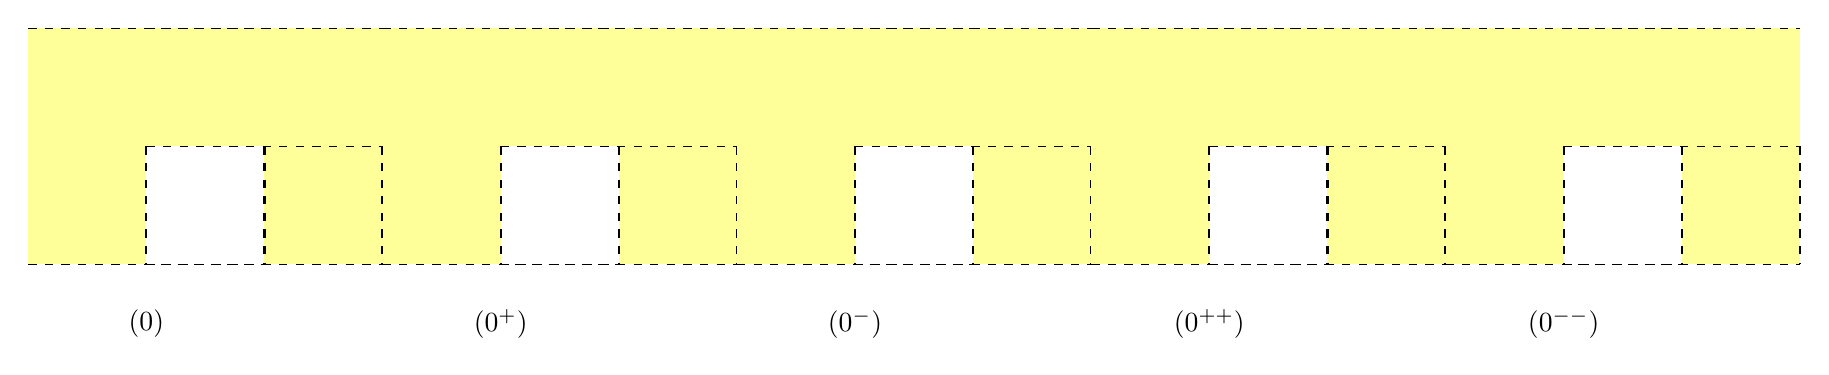
\begin{tikzpicture}[scale=1.5]
        % Define colors
        \definecolor{myyellow}{RGB}{255, 255, 153}
        \definecolor{mygray}{RGB}{204, 204, 204}
        
        % Draw the yellow region
        \fill[myyellow] (0,0) -- (1,0) -- (1,1) -- (0,1) -- cycle;
        \fill[myyellow] (0,1) -- (-1,1) -- (-1,-1) -- (0,-1) -- cycle;
        \fill[myyellow] (1,0) -- (2,0) -- (2,1) -- (1,1) -- cycle;
        \fill[myyellow] (1,1) -- (2,1) -- (2,-1) -- (1,-1) -- cycle;
        
        % Draw the dashed lines
        \draw[dashed] (0,0) -- (2,0);
        \draw[dashed] (0,1) -- (2,1);
        \draw[dashed] (0,-1) -- (2,-1);
        \draw[dashed] (-1,1) -- (1,1);
        \draw[dashed] (-1,-1) -- (1,-1);
        
        % Draw the black dashed line
        \draw[dashed, thick] (0,0) -- (0,-1);
        \draw[dashed, thick] (1,0) -- (1,-1);
        \draw[dashed, thick] (2,0) -- (2,-1);
        
        % Label the region
        \node at (0,-1.5) {$(0)$};
        
        % Draw the second diagram
        \begin{scope}[xshift=3cm]
            % Draw the yellow region
            \fill[myyellow] (0,0) -- (1,0) -- (1,1) -- (0,1) -- cycle;
            \fill[myyellow] (0,1) -- (-1,1) -- (-1,-1) -- (0,-1) -- cycle;
            \fill[myyellow] (1,0) -- (2,0) -- (2,1) -- (1,1) -- cycle;
            \fill[myyellow] (1,1) -- (2,1) -- (2,-1) -- (1,-1) -- cycle;
            
            % Draw the dashed lines
            \draw[dashed] (0,0) -- (2,0);
            \draw[dashed] (0,1) -- (2,1);
            \draw[dashed] (0,-1) -- (2,-1);
            \draw[dashed] (-1,1) -- (1,1);
            \draw[dashed] (-1,-1) -- (1,-1);
            
            % Draw the black dashed line
            \draw[dashed, thick] (0,0) -- (0,-1);
            \draw[dashed, thick] (1,0) -- (1,-1);
            \draw[dashed, thick] (2,0) -- (2,-1);
            
            % Label the region
            \node at (0,-1.5) {$(0^{+})$};
        \end{scope}
        
        % Draw the third diagram
        \begin{scope}[xshift=6cm]
            % Draw the yellow region
            \fill[myyellow] (0,0) -- (1,0) -- (1,1) -- (0,1) -- cycle;
            \fill[myyellow] (0,1) -- (-1,1) -- (-1,-1) -- (0,-1) -- cycle;
            \fill[myyellow] (1,0) -- (2,0) -- (2,1) -- (1,1) -- cycle;
            \fill[myyellow] (1,1) -- (2,1) -- (2,-1) -- (1,-1) -- cycle;
            
            % Draw the dashed lines
            \draw[dashed] (0,0) -- (2,0);
            \draw[dashed] (0,1) -- (2,1);
            \draw[dashed] (0,-1) -- (2,-1);
            \draw[dashed] (-1,1) -- (1,1);
            \draw[dashed] (-1,-1) -- (1,-1);
            
            % Draw the black dashed line
            \draw[dashed, thick] (0,0) -- (0,-1);
            \draw[dashed, thick] (1,0) -- (1,-1);
            \draw[dashed, thick] (2,0) -- (2,-1);
            
            % Label the region
            \node at (0,-1.5) {$(0^{-})$};
        \end{scope}
        
        % Draw the fourth diagram
        \begin{scope}[xshift=9cm]
            % Draw the yellow region
            \fill[myyellow] (0,0) -- (1,0) -- (1,1) -- (0,1) -- cycle;
            \fill[myyellow] (0,1) -- (-1,1) -- (-1,-1) -- (0,-1) -- cycle;
            \fill[myyellow] (1,0) -- (2,0) -- (2,1) -- (1,1) -- cycle;
            \fill[myyellow] (1,1) -- (2,1) -- (2,-1) -- (1,-1) -- cycle;
            
            % Draw the dashed lines
            \draw[dashed] (0,0) -- (2,0);
            \draw[dashed] (0,1) -- (2,1);
            \draw[dashed] (0,-1) -- (2,-1);
            \draw[dashed] (-1,1) -- (1,1);
            \draw[dashed] (-1,-1) -- (1,-1);
            
            % Draw the black dashed line
            \draw[dashed, thick] (0,0) -- (0,-1);
            \draw[dashed, thick] (1,0) -- (1,-1);
            \draw[dashed, thick] (2,0) -- (2,-1);
            
            % Label the region
            \node at (0,-1.5) {$(0^{++})$};
        \end{scope}
        
        % Draw the fifth diagram
        \begin{scope}[xshift=12cm]
            % Draw the yellow region
            \fill[myyellow] (0,0) -- (1,0) -- (1,1) -- (0,1) -- cycle;
            \fill[myyellow] (0,1) -- (-1,1) -- (-1,-1) -- (0,-1) -- cycle;
            \fill[myyellow] (1,0) -- (2,0) -- (2,1) -- (1,1) -- cycle;
            \fill[myyellow] (1,1) -- (2,1) -- (2,-1) -- (1,-1) -- cycle;
            
            % Draw the dashed lines
            \draw[dashed] (0,0) -- (2,0);
            \draw[dashed] (0,1) -- (2,1);
            \draw[dashed] (0,-1) -- (2,-1);
            \draw[dashed] (-1,1) -- (1,1);
            \draw[dashed] (-1,-1) -- (1,-1);
            
            % Draw the black dashed line
            \draw[dashed, thick] (0,0) -- (0,-1);
            \draw[dashed, thick] (1,0) -- (1,-1);
            \draw[dashed, thick] (2,0) -- (2,-1);
            
            % Label the region
            \node at (0,-1.5) {$(0^{--})$};
        \end{scope}
    \end{tikzpicture}
\end{figure}

\end{document}